\documentclass[xcolor=dvipsnames,table]{beamer}

\usepackage{latexsym}
\usepackage[utf8]{inputenc}
\usepackage[brazil]{babel}
\usepackage{amssymb}
\usepackage{amsmath}
\usepackage{stmaryrd}
\usepackage{fancybox}
\usepackage{datetime}
\usepackage[T1]{fontenc}
\usepackage{graphicx}
\usepackage{graphics}
\usepackage{url}
\usepackage{algorithmic}
\usepackage{algorithm}
\usepackage{acronym}
\usepackage{array}

\newtheorem{definicao}{Definio}
\newcommand{\tab}{\hspace*{2em}}

\mode<presentation>
{
  \definecolor{colortexto}{RGB}{0,0,0}
 
  \setbeamertemplate{background canvas}[vertical shading][ bottom=white!10,top=white!10]
  \setbeamercolor{normal text}{fg=colortexto} 

  \usetheme{Warsaw}
}

\title{Apresentação da disciplina} 

\author{
  Esdras Lins Bispo Jr. \\ \url{bispojr@ufg.br}
  } 
 \institute{
  Teoria da Computação \\Bacharelado em Ciência da Computação}
\date{\textbf{27 de março de 2018} }

\logo{
\includegraphics[width=1cm]{images/ufgJataiLogo.png}}

\begin{document}

	\begin{frame}
		\titlepage
	\end{frame}

	\begin{frame}{Plano de Aula}
		\tableofcontents
		%\tableofcontents[hideallsubsections]
	\end{frame}
	
	\section{Sobre a Disciplina}
	\subsection{Professor}
	\begin{frame}{Professor}
		\begin{columns}
			\column{.4\textwidth}  		
		  		\begin{center}
		    		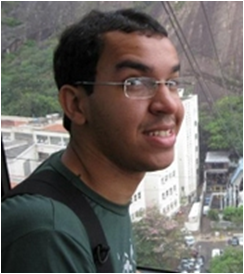
\includegraphics[height=.5\textheight]{images/esdras.png}
		  		\end{center}
			\column{.6 \textwidth}  		
				\begin{block}{Formação}
					\begin{center}
						{\normalsize {\bf Bacharel} em Sistemas de Informação\\
						{\bf Mestre} em Representação Conhecimento (IA)}
					\end{center}
				\end{block}		  		
		  		\begin{block}{Quem?}
		  			\begin{center}
						{\bf Esdras Lins Bispo Junior} \\ Recife, Pernambuco.
					\end{center}
				\end{block}
		\end{columns}
	\end{frame}
	
	\subsection{Informações Importantes}
	\begin{frame}{Informações Importantes}
		\begin{block}{Professor}
			\begin{itemize}
				\item Esdras Lins Bispo Jr.
				\item \url{bispojr@ufg.br}
				\item Sala 18, 1º Andar (Bloco Novo dos Professores)
			\end{itemize}
		\end{block}
	\end{frame}	
	
	\begin{frame}{Informações Importantes}
		\begin{block}{Disciplina}
			\begin{itemize}
				\item Teoria da Computação
				\item 09h30-11h10 (Segunda, [CA2, Sala 05])\\
					  13h30-15h10 (Quinta, [CA2, Sala 11])
				\item Dúvidas: 07h30 - 09h00 (Segunda)\\
					  {\color{red}[é necessário confirmação comigo]}
				\item Grupo: \url{facebook.com/groups/teocomp.ufj.2018.1/}
				\item Repositório: \url{github.com/bispojr/teoria-computacao}
			\end{itemize}
		\end{block}
	\end{frame}
	
	\begin{frame}{Informações Importantes}
		\begin{block}{Metodologia}
			\begin{itemize}
				\item Aulas expositivas utilizando quadro negro (ou branco) e DataShow;
				\item Atendimento individual ou em grupos;
				\item Aplicação de listas de exercícios;
				\item Tempo de Aula: 50 minutos.
			\end{itemize}
		\end{block}
	\end{frame}
	
	\subsection{Instrumentos de Avaliação}
	\begin{frame}{Instrumentos de Avaliação}
		\begin{block}{Lista de Exercícios}
			\begin{itemize}
				\item Encontros de 30 minutos para a apresentação das respostas;
				\item Para cada questão, 40\% corresponde à resposta escrita e \\60\% à apresentação individual para o professor;
				\item O somatório da pontuação obtida por todas as questões compreende a pontuação total da lista de exercícios;
				\item É possível refazer o exercício a qualquer momento com o propósito de melhorar a pontuação referente àquele exercício.
			\end{itemize}
		\end{block}
	\end{frame}
	
	\begin{frame}{Informações Importantes}
		\begin{block}{Conteúdo do Curso}
			\begin{enumerate}
				\item Introdução à Teoria da Computação;
				\item Modelos de Computação;
				\item Problemas decidíveis;
				\item Problemas indecidíveis;
				\item Complexidade de tempo;
				\item NP-Completude;
				\item Tópicos Avançados.
			\end{enumerate}
		\end{block}
	\end{frame}
	
	\begin{frame}
		\titlepage
	\end{frame}
	
\end{document}